\documentclass{article}
\usepackage[utf8]{inputenc}
\usepackage{amsmath}
\usepackage{graphicx}
\renewcommand\thesection{\alph{section}}
\title{BIOS13 - Question 3}
\author{Pham Xuan Huy Nguyen}
\begin{document}
\maketitle
\section{Workers population}
The equation \(\frac{dW}{dt}=rW\) can also be expressed as:
\[\frac{1}{W}dW=rdt \]
Integrate to get the equation of individuals:
\[\int{\frac{1}{W}dW}=\int{rdt}\]
\begin{equation}\label{1}
   \Leftrightarrow ln(W)=rt + C
\end{equation}
Initially, we have W=1 (the colony start with 1) at time t=0, we get:
\[ln(1)=r*0 + C\]
\begin{equation}\label{2}
    \Leftrightarrow C=0
\end{equation}
Substitute (\ref{2}) into (\ref{1}), we have:
\[lnW=rt \]
\[\Leftrightarrow W=e^{rt} \]
We have an equation of population of worker \textit{W} corresponding to time \textit{t}, thus at time \textit{t\textsubscript{s}}, we have:
\begin{equation}\label{3}
W(t\textsubscript{s})=e^{rt\textsubscript{s}}
\end{equation}
\section{Number of queens}
The number of queens function \(\frac{dQ}{dt}=cW\) can also be expressed as:
\[dQ=cWdt \]
The queens will be produced after switching time \textit{t\textsubscript{s}}, thus the number of queens at time \textit{T} is the result of:
\[Q\textsubscript{T} = \int_{t\textsubscript{s}}^{T} cW \,dt \]
\begin{equation}\label{4}
\Leftrightarrow Q\textsubscript{T} =cW(T-t\textsubscript{s})
\end{equation}
From (\ref{3}), (\ref{4}) can be written as:
\begin{equation}\label{5}
    \Leftrightarrow Q\textsubscript{T} =ce^{rt\textsubscript{s}}(T-t\textsubscript{s})
\end{equation}
\section{Optimal switching time}
Find the first derivative of (\ref{5}) with respect to \textit{t\textsubscript{s}} :
\[Q\textsubscript{T}'=cre^{rt\textsubscript{s}}(T-t\textsubscript{s})-ce^{rt\textsubscript{s}}\]
Find the value of \textit{t\textsubscript{s}} when \textit{Q\textsubscript{T}'}=0
\[ce^{rt\textsubscript{s}}(r(T-t\textsubscript{s})-1)=0\]
\[\Leftrightarrow ce^{rt\textsubscript{s}}=0 	\lor r(T-t\textsubscript{s})-1 =0 \]
\begin{equation}\label{6}
 \Leftrightarrow  t\textsubscript{s}=T-\frac{1}{r}   
\end{equation}
Find the second derivative of \textit{Q\textsubscript{T}} with respect to \textit{t\textsubscript{s}} : 
\[Q\textsubscript{T}''=cr^{2}e^{rt\textsubscript{s}}(T-t\textsubscript{s})-cre^{rt\textsubscript{s}}-cre^{rt\textsubscript{s}}\]
\[\Leftrightarrow Q\textsubscript{T}''=r(cre^{rt\textsubscript{s}}((T-t\textsubscript{s})-ce^{rt\textsubscript{s}}-ce^{rt\textsubscript{s}})\]
\begin{equation}\label{7}
    \Leftrightarrow Q\textsubscript{T}''=r(Q\textsubscript{T}'-ce^{rt\textsubscript{s}})
\end{equation}
We know that when substitute (\ref{6}) to (\ref{7}), \textit{Q\textsubscript{T}'} will be equal to 0, thus we have:
\[Q\textsubscript{T}''=-rce^{r(T-\frac{1}{r})}\]
Since \textit{r,c} is a positive number, and \(e^{r(T-\frac{1}{r})}\) is never smaller than 0, \textit{Q\textsubscript{T}''} $<$ 0.\\
Thus there is a local maxima of \textit{Q\textsubscript{T}}  when \(t\textsubscript{s}=T-\frac{1}{r}\)

\section{Extend model}
Let's call \textit{a} is the dying rate of workers bee, and \textit{b} is the dying rate of queen bees.\\
Before \textit{t\textsubscript{s}}, the growth of worker bees is:
\[\frac{dW}{dt}=rW-aW\]
After \textit{t\textsubscript{s}}, worker bees stop reproducing and start to die:
\[\frac{dW}{dt}=-aW\]
Before \textit{t\textsubscript{s}}, there is no reproduction of queen bees:
\[\frac{dQ}{dt}=0\]
After \textit{t\textsubscript{s}}, queen bees start reproducing with a rate depends on the number of worker and dying at the same time:
\[\frac{dQ}{dt}=cW-bQ\]

\section{R script}
\begin{verbatim}
rm(list=ls())
library(deSolve)
Q3e = function(ts,T,r,c,a,b){
  WQ = function(t,wp,P){
    W = wp[1]
    Q = wp[2]
    if (t<=ts) {
      dWdt = P$r*W - P$a*W
      dQdt = 0
    } else if (t>ts) {
      dWdt = -P$a*W
      dQdt = P$c*W - P$b*Q
    }
    return(list(c(dWdt,dQdt)))
  }
  timevec = seq(0,T,by=1)
  P = list(r=r,c=c,a=a,b=b)
  wp0 = c(W=1,Q=0)
  out = ode(y=wp0,func=WQ,parms=P,times=timevec)
  
  time <- out[,'time']
  w <- out[,'W']
  q <- out[,'Q']
  plot( time, w, type='l', col='blue',xlim=c(0,100),
        ylim=c(0,max(w)),ylab="W,Q",xlab="t")
  lines( time, q, col='red')
  legend("topleft", legend = c("Worker", "Queen"),
         lwd = 1, col = c("blue", "red"), cex=0.6)
}
Q3e(60,100,0.08,0.01,0.01,0.001)
\end{verbatim}
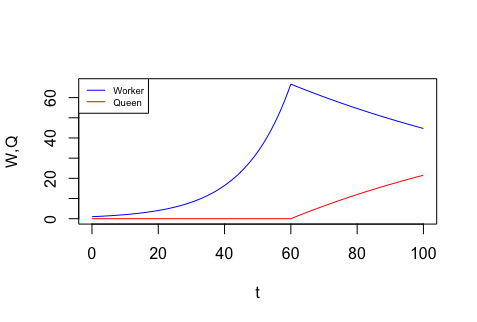
\includegraphics[width=\textwidth]{images/3e.png}
The plot is illustrated by the following code \textit{Q3e(60,100,0.08,0.01,0.01,0.001)}

\end{document}

